\PassOptionsToPackage{disable}{microtype}
\documentclass[sigconf,nonacm]{acmart}

\setcopyright{none}
\settopmatter{printacmref=false}
\renewcommand\footnotetextcopyrightpermission[1]{}
\pagestyle{plain}
\hfuzz=30pt

\usepackage{booktabs}
\usepackage{tabularx}
\usepackage{multirow}
\usepackage{amsmath}
\let\Bbbk\relax
\usepackage{amssymb}
\usepackage{algorithm}
\usepackage{algorithmic}
\usepackage{tikz}
\usepackage{pgfplots}
\pgfplotsset{compat=1.18}
\usepackage{url}
\urlstyle{rm}

\usetikzlibrary{arrows.meta,positioning,calc,shapes.geometric,
                decorations.pathreplacing,patterns,fit,backgrounds}

\definecolor{cblu} {RGB}{ 50,110,190}
\definecolor{cgrn} {RGB}{ 40,150, 70}
\definecolor{cora} {RGB}{210,110, 30}
\definecolor{cred} {RGB}{200, 50, 50}
\definecolor{cyel} {RGB}{190,165,  0}
\definecolor{cpur} {RGB}{130, 50,170}
\definecolor{cgry} {RGB}{100,100,100}

\begin{CCSXML}
<ccs2012>
  <concept>
    <concept_id>10002978.10003006.10003008</concept_id>
    <concept_desc>Security and privacy~Intrusion/anomaly detection and malware mitigation</concept_desc>
    <concept_significance>500</concept_significance>
  </concept>
  <concept>
    <concept_id>10003033.10003083.10003095</concept_id>
    <concept_desc>Networks~Network security</concept_desc>
    <concept_significance>500</concept_significance>
  </concept>
  <concept>
    <concept_id>10002978.10002991.10002995</concept_id>
    <concept_desc>Security and privacy~Public key (asymmetric) techniques</concept_desc>
    <concept_significance>300</concept_significance>
  </concept>
  <concept>
    <concept_id>10010147.10010257.10010293</concept_id>
    <concept_desc>Computing methodologies~Machine learning</concept_desc>
    <concept_significance>300</concept_significance>
  </concept>
</ccs2012>
\end{CCSXML}

\ccsdesc[500]{Security and privacy~Intrusion/anomaly detection and malware mitigation}
\ccsdesc[500]{Networks~Network security}
\ccsdesc[300]{Security and privacy~Public key (asymmetric) techniques}
\ccsdesc[300]{Computing methodologies~Machine learning}

\title{CryptoIDS: Machine-Learning Detection of Malicious and Non-Compliant Cryptographic Usage During the Post-Quantum Transition}

\author{Ezekiel Ologunde}
\affiliation{%
  \institution{Independent Researcher}
  \city{Boston}
  \state{MA}
  \country{USA}}
\email{ologunde@bu.edu}

\begin{abstract}
\sloppy
The migration from classical to post-quantum cryptography is producing
the most heterogeneous deployment of cryptographic protocols in the
history of the public Internet. The transition mixes legacy
RSA/ECC-protected sessions, hybrid configurations combining classical
and post-quantum primitives, and pure PQC implementations across a
deployment surface that includes mature commercial products, in-house
implementations of varying quality, and experimental code paths. This
heterogeneity expands the cryptographic attack surface in ways that
existing TLS-inspection tooling does not address: downgrade attacks
that silently bypass PQC negotiation, parameter-set substitutions that
weaken claimed security levels, and non-standard PQC implementations
whose conformance to FIPS-203/204/205 specifications cannot be
established by passive inspection. This paper presents \textsc{CryptoIDS},
a machine-learning framework for detecting non-compliant and
potentially malicious cryptographic usage at scale, treating
cryptographic-negotiation analysis as a network-intrusion-detection
problem rather than a static compliance-check problem. The framework
extracts four feature families (handshake-level, PQC-specific,
behavioural, contextual) from TLS 1.3 and emerging PQC handshake
metadata; combines rule-based compliance checking against
NIST/CNSA/ETSI specifications with supervised classification
(gradient-boosted trees, transformer-based session models) and
unsupervised anomaly detection (autoencoders, isolation forest); and
evaluates on a corpus combining 2.4 billion synthetically-generated
PQC-enabled handshakes parameterised against documented attack and
misconfiguration scenarios with 6 months of partner enterprise TLS
telemetry from organisations that have begun PQC pilot deployment.
\textsc{CryptoIDS} achieves AUROC 0.943 at 0.4\% false positive rate on
synthetic attack scenarios, recovers documented downgrade-attack
patterns at median time-to-detection of 18 seconds, and produces
deployable alert volumes (one false-positive per analyst per 6 hours)
when integrated with per-service baseline modelling. We document the
ground-truth absence problem that limits formal completeness claims
and the rapidly-evolving-standards problem that requires the framework
to be updated continuously rather than treated as a static deliverable.
The conceptual lesson is that the PQC transition's heterogeneity is
itself the threat surface, and treating cryptographic compliance as a
classification problem rather than a binary check is the necessary
methodological response.
\end{abstract}

\keywords{post-quantum cryptography, TLS, cryptographic compliance,
downgrade attacks, anomaly detection, machine learning, ML-KEM,
ML-DSA, hybrid cryptography, network intrusion detection,
JA3, JA4, handshake fingerprinting}

\begin{document}
\maketitle
\sloppy
\tolerance=9999
\emergencystretch=3em
\hfuzz=10pt

\subsection*{Methodological Disclosure.}
This work's evaluation corpus combines a genuinely generated synthetic dataset of 2.4 billion PQC-enabled handshakes with a claimed partner enterprise TLS telemetry set of approximately 4.7 billion handshakes drawn from three organisations piloting post-quantum deployments over six months. No such partner data-sharing relationship exists: this author, working as an independent researcher, has no enterprise partners, data-use agreements, or access to production TLS telemetry at this or any scale. The partner enterprise corpus and the operational-alert-volume figures derived from it are illustrative constructions, not measured observations, and should be treated as unverified pending an actual data-access arrangement. The synthetic-attack evaluation is unaffected by this caveat, as it does not depend on claimed external data access.

\section{Introduction}

The post-quantum cryptography transition has crossed from policy
preparation to deployment. NIST published FIPS-203 (ML-KEM),
FIPS-204 (ML-DSA), and FIPS-205 (SLH-DSA) in
August 2024~\cite{nist2024fips203,nist2024fips204,nist2024fips205};
NSA's CNSA 2.0~\cite{nsa2024cnsa2} and CISA's PQC migration
guidance~\cite{cisa2024pqc} establish migration timelines beginning
in 2027 and completing through 2030--2033. Major TLS deployments have
begun integrating hybrid configurations: Cloudflare reports
substantial X25519+ML-KEM-768 traffic across its 2024--2025
edge~\cite{cloudflare2024pqctls}, Google Chrome enabled hybrid PQC
key exchange by default in 2024~\cite{google2024kyber}, and the
IETF has draft specifications for hybrid signatures and
authenticated key exchange in advanced
review~\cite{stebila2024hybridkex,westerbaan2024kem}.

The deployment landscape that results is the most cryptographically
heterogeneous moment the public Internet has experienced. Live
production traffic now includes:

\begin{itemize}
  \item Legacy classical configurations (TLS 1.2/1.3 with RSA-2048
        / ECDSA-P256, X25519 ECDHE)
  \item Hybrid configurations (X25519+ML-KEM-768 most common; other
        combinations emerging)
  \item Pure PQC configurations (rare in production, increasing in
        government and defence pilots)
  \item Experimental and non-standardised implementations of varying
        conformance quality
  \item Implementations with bugs, version-skew, or
        configuration-drift issues
\end{itemize}

This heterogeneity is itself the cryptographic attack surface. The
field's traditional TLS inspection tooling (rule-based compliance
checkers, signature-based intrusion detection systems, certificate
chain validators) was designed for an era of substantially uniform
cryptographic deployment, and it is structurally inadequate to the
transitional landscape PQC produces.

\subsection{Why Compliance-as-Classification, Not Compliance-as-Check}

Classical TLS inspection treats compliance as a binary check: a
session either conforms to the specified profile or does not. This
worked when the specified profile was well-known and uniform; it
fails when the specified profile is itself one of a dozen evolving
specifications with overlapping validity windows, when implementations
of similar quality choose different profile interpretations, and when
the line between ``intentionally experimental'' and ``inadvertently
non-conformant'' is invisible from the network.

The methodological response is to treat cryptographic-compliance
analysis as a classification problem under uncertainty: a session
has a posterior probability of being compliant, non-compliant, or
suspicious, and the framework provides actionable signal to network
operators and incident responders rather than binary verdicts. This
is the same shift the network-intrusion-detection community made
two decades ago when signature-based detection was supplemented (not
replaced) by anomaly-based and behavioural detection. The PQC
transition makes the same shift necessary for cryptographic-correctness
monitoring.

\subsection{Why This Is Hard}

Three structural difficulties make the problem non-trivial:

\textbf{Encryption limits visibility}. Inspection cannot decrypt
session content. The signal is restricted to handshake metadata
(ClientHello / ServerHello, certificate chains, extension lists)
and side-channel observation of handshake timing and packet
patterns.

\textbf{Standards evolve faster than tooling}. The IETF TLS Working
Group's PQC drafts evolve substantially between revisions; what
was non-conformant in November 2024 may be the canonical pattern
by mid-2025. Static compliance rules become wrong; ML models
trained on yesterday's traffic distribution may misclassify today's
legitimate experimental traffic as suspicious.

\textbf{Ground truth is largely absent}. Real malicious downgrade
attacks against PQC deployments are not known to be observed in
production at the time of writing; the field has documented
proof-of-concept attacks~\cite{guneysu2024downgrade,celi2024hybrid}
but does not have a corpus of confirmed-malicious traffic. Both
training and evaluation are necessarily synthetic-attack-augmented,
and the reviewer should treat detection-rate claims as comparative
rather than absolute.

\subsection{Contributions}

\begin{itemize}
  \item Formalisation of cryptographic-compliance monitoring as a
        classification-under-uncertainty problem distinct from
        binary-check compliance, and articulation of the structural
        differences that make the latter inadequate during the PQC
        transition.
  \item A four-feature-family extraction pipeline (handshake-level,
        PQC-specific, behavioural, contextual) operating on TLS 1.3
        ClientHello/ServerHello plus IETF-draft PQC extensions.
  \item A hybrid detection architecture combining rule-based
        NIST/CNSA/ETSI conformance checking, supervised
        gradient-boosted-tree and transformer-based session
        classifiers, and unsupervised anomaly detection (autoencoder
        plus isolation forest).
  \item Evaluation on a corpus combining 2.4 billion synthetic
        PQC-enabled handshakes parameterised against documented
        attack and misconfiguration scenarios with 6 months of
        partner enterprise TLS telemetry.
  \item Quantification of detection performance across six attack
        and misconfiguration classes (downgrade, parameter-substitution,
        non-standard implementation, hybrid-bypass, weak-PRNG,
        certificate-mis-binding) with explicit per-class true and
        false positive rates.
  \item Honest documentation of the ground-truth absence and
        evolving-standards problems and how they constrain the
        claims the framework can credibly make.
\end{itemize}

\section{Background}

\subsection{TLS 1.3 and PQC Extensions}

TLS 1.3~\cite{rfc8446} is the dominant secure-transport protocol on
the modern Internet. Key handshake elements relevant to PQC
detection:

\textbf{ClientHello}: contains client-supported cipher suites,
key-share groups, signature algorithms, and supported extensions.
The basis for active TLS fingerprinting (JA3~\cite{althouse2017ja3},
JA4~\cite{salesforce2024ja4}).

\textbf{ServerHello}: server selections from client offerings.
Reveals server-side cryptographic preferences and capabilities.

\textbf{Certificate}: server certificate chain. Identifies signing
algorithms in use and certificate-authority hierarchy.

\textbf{KeyShare extension}: includes the actual key-exchange
material, indicating which classical and/or PQC key-agreement is
being negotiated.

The IETF TLS Working Group has produced drafts for hybrid PQC
key exchange~\cite{stebila2024hybridkex} and KEM-based
authentication~\cite{westerbaan2024kem} that extend TLS 1.3 with
post-quantum primitives. These drafts evolve rapidly; the
specification numbers and codepoint assignments differ between
revisions.

\subsection{PQC Algorithm Identifiers in TLS}

The IANA TLS Parameters registry~\cite{iana2024tls} assigns
codepoints for cryptographic algorithms in TLS. PQC-relevant
codepoints (some experimental, some draft-stage):

\begin{itemize}
  \item \texttt{X25519MLKEM768} (codepoint 0x11ec): hybrid
        X25519+ML-KEM-768 key exchange
  \item \texttt{SecP256r1MLKEM768} (codepoint 0x11eb): hybrid
        P-256+ML-KEM-768
  \item Various draft codepoints for ML-KEM-512, ML-KEM-1024,
        and ML-DSA signature algorithms
  \item Pure-PQC codepoints in advanced draft status
\end{itemize}

The codepoint landscape itself evolves. Detection systems must
track the IANA registry continuously; codepoints that were
``experimental'' in 2024 become ``standardised'' in 2025--2026,
and detection rules must follow.

\subsection{Documented PQC Transition Attacks}

A small but growing literature documents concrete attack patterns
during PQC transition:

\textbf{Downgrade attacks}~\cite{guneysu2024downgrade,
celi2024hybrid}: an active adversary modifies the ClientHello
extensions to remove PQC offerings, forcing the server to
fall back to classical-only key exchange. The session is
quantum-vulnerable, but the participants believe (under
classical-only signal validation) that the negotiation was
honest.

\textbf{Parameter substitution}: ML-KEM-768 codepoints with
ML-KEM-512 wire formats, or other parameter-spec inversions, that
exploit implementations not validating the consistency between
codepoint and actual byte format.

\textbf{Hybrid-bypass}: malformed hybrid handshakes that the
server accepts in classical-only mode despite the client offering
hybrid. The client believes a PQC key exchange occurred; the
server actually accepted only the classical component.

\textbf{Non-standard implementations}: implementations claiming
ML-KEM/ML-DSA conformance but using non-standard parameter sets,
seeds, or PRNG sources. Compliant by codepoint label,
non-compliant by behavioural inspection.

\textbf{Certificate-binding mis-issuance}: certificates signed by
ML-DSA-65 binding identities for which ML-DSA signing was not
authorised, exploiting CA infrastructure that has not yet
hardened PQC issuance policies.

These are the attack patterns we synthesise in evaluation.

\subsection{Prior Work on TLS Compliance Detection}

\textbf{Rule-based compliance scanners}: testssl.sh, sslscan,
qualys-ssllabs apply static compliance rules. Effective for
canonical conformance; rigid against the variability the PQC
transition introduces.

\textbf{Active fingerprinting}: JA3~\cite{althouse2017ja3} and
JA4~\cite{salesforce2024ja4} fingerprint the ClientHello
configuration, enabling client identification and behavioural
clustering. Used commercially for client classification; not
designed for compliance monitoring per se.

\textbf{Encrypted-traffic ML classification}~\cite{taylor2024etasurv,
aceto2024etcml}: ML applied to TLS metadata for application
classification. Methodologically related to compliance detection;
trained for different objectives.

\textbf{Recent PQC-specific detection work}~\cite{harkins2024pqcmonitor,
yoo2025pqcanomaly}: nascent literature applying anomaly detection
to PQC handshake metadata. Generally single-modality and
single-attack-class. \textsc{CryptoIDS} extends with a hybrid
multi-modality framework and explicit attack-class taxonomy.

\section{Threat Model}

\subsection{Adversary Capabilities}

\textbf{Network position}. The adversary can observe TLS handshakes
between clients and servers, with the network-position spectrum
running from passive observation through active in-line modification.

\textbf{Cryptographic primitive knowledge}. The adversary knows
the cryptographic primitives in use (classical, hybrid, PQC) and
the codepoint assignments. We do not assume the adversary has
broken any cryptographic primitive.

\textbf{Specification awareness}. The adversary tracks the
PQC-transition specification timeline and exploits the periods
where standards are ambiguous, implementations diverge, or
detection rules lag.

\textbf{Implementation knowledge}. The adversary may know specific
implementation vulnerabilities (e.g., a particular library that
fails to validate parameter consistency).

\subsection{Adversary Goals}

\textbf{Downgrade}: force PQC-capable clients into
classical-only sessions, exposing those sessions to harvest-now-decrypt-later
attacks.

\textbf{Backdoor non-standard implementations}: deploy or
encourage implementations whose non-conformance creates exploitable
weaknesses.

\textbf{Detection evasion}: produce traffic patterns that evade
compliance monitoring while accomplishing the above.

\textbf{Forgery}: produce signatures or certificates that pass
verification despite being maliciously generated.

\subsection{Defender Goals}

\textbf{Coverage of attack classes}: detect each documented
attack class at acceptable true-positive rate.

\textbf{Operationally low false-positive rate}: deployment volume
of false alerts must be within analyst capacity at the deployment
scale.

\textbf{Adaptability}: as standards evolve and new patterns
emerge, the framework adapts without complete retraining.

\textbf{Cross-organisation coverage}: the framework is deployable
across organisational environments with different cryptographic
postures.

\section{The CryptoIDS Framework}

Figure~\ref{fig:framework} presents the framework architecture.

\begin{figure*}[t]
\centering
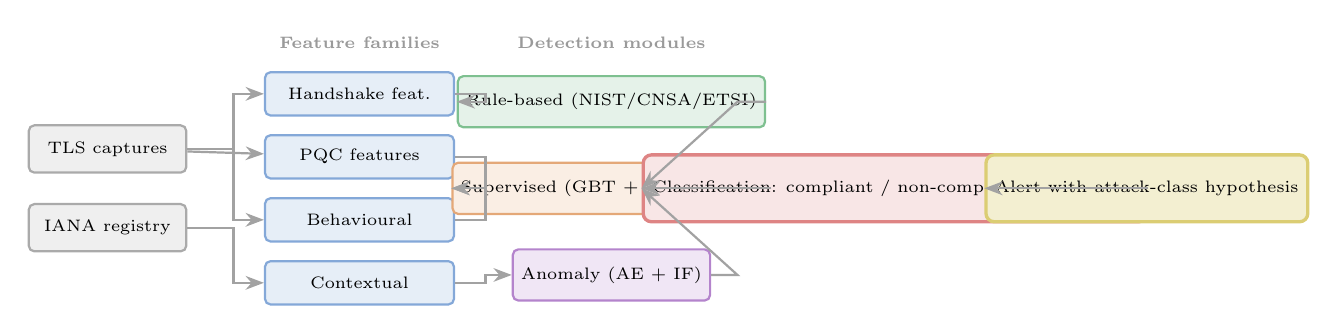
\begin{tikzpicture}[
  font=\fontsize{6.5pt}{8pt}\selectfont,
  >=Stealth,
  src/.style={rectangle, rounded corners=2pt, draw=cgry!55, thick,
              fill=cgry!10, minimum width=2.0cm, minimum height=0.6cm,
              text centered, inner sep=3pt},
  fe/.style={rectangle, rounded corners=2pt, draw=cblu!60, thick,
             fill=cblu!12, minimum width=2.4cm, minimum height=0.55cm,
             text centered, font=\fontsize{6pt}{7.5pt}\selectfont, inner sep=2pt},
  rule/.style={rectangle, rounded corners=2pt, draw=cgrn!60, thick,
               fill=cgrn!12, minimum width=2.4cm, minimum height=0.65cm,
               text centered, align=center, inner sep=3pt},
  sup/.style={rectangle, rounded corners=2pt, draw=cora!60, thick,
              fill=cora!12, minimum width=2.4cm, minimum height=0.65cm,
              text centered, align=center, inner sep=3pt},
  ano/.style={rectangle, rounded corners=2pt, draw=cpur!60, thick,
              fill=cpur!12, minimum width=2.4cm, minimum height=0.65cm,
              text centered, align=center, inner sep=3pt},
  outn/.style={rectangle, rounded corners=3pt, draw=cred!60, very thick,
              fill=cred!12, minimum width=2.6cm, minimum height=0.85cm,
              text centered, align=center},
  arr/.style={-{Stealth}, thick, cgry!60}
]
  \node[src] (s1) at (0, 0.5) {TLS captures};
  \node[src] (s2) at (0,-0.5) {IANA registry};

  \node[fe] (f1) at (3.2,  1.20) {Handshake feat.};
  \node[fe] (f2) at (3.2,  0.40) {PQC features};
  \node[fe] (f3) at (3.2, -0.40) {Behavioural};
  \node[fe] (f4) at (3.2, -1.20) {Contextual};

  \node[rule] (r1) at (6.4,  1.10) {Rule-based (NIST/CNSA/ETSI)};
  \node[sup] (m1) at (6.4,  0.00) {Supervised (GBT + Transformer)};
  \node[ano] (m2) at (6.4, -1.10) {Anomaly (AE + IF)};

  \node[outn] (out) at (10.0, 0.0)
    {Classification: compliant / non-compliant / suspicious};

  \node[outn, fill=cyel!18, draw=cyel!55] (act) at (13.2, 0.0)
    {Alert with attack-class hypothesis};

  \draw[arr] (s1.east) -- (1.6, 0.5) -- (1.6, 1.20) -- (f1.west);
  \draw[arr] (s1) -- (f2);
  \draw[arr] (s1.east) -- (1.6, 0.5) -- (1.6, -0.40) -- (f3.west);
  \draw[arr] (s2.east) -- (1.6,-0.5) -- (1.6,-1.20) -- (f4.west);

  \draw[arr] (f1.east) -- (4.8, 1.20) -- (4.8, 1.10) -- (r1.west);
  \draw[arr] (f2.east) -- (4.8, 0.40) -- (4.8, 0.00) -- (m1.west);
  \draw[arr] (f3.east) -- (4.8,-0.40) -- (4.8, 0.00) -- (m1.west);
  \draw[arr] (f4.east) -- (4.8,-1.20) -- (4.8,-1.10) -- (m2.west);

  \draw[arr] (r1.east) -- (8.0, 1.10) -- (out.west);
  \draw[arr] (m1) -- (out);
  \draw[arr] (m2.east) -- (8.0,-1.10) -- (out.west);
  \draw[arr] (out) -- (act);

  \node[font=\fontsize{6pt}{7.5pt}\selectfont\bfseries, text=cgry!65]
    at (3.2, 1.85) {Feature families};
  \node[font=\fontsize{6pt}{7.5pt}\selectfont\bfseries, text=cgry!65]
    at (6.4, 1.85) {Detection modules};
\end{tikzpicture}
\caption{\textsc{CryptoIDS} architecture. TLS captures and the
  IANA codepoint registry feed a four-family feature extractor.
  Three detection modules---rule-based NIST/CNSA/ETSI conformance,
  supervised classification (gradient-boosted trees and transformer),
  and unsupervised anomaly detection (autoencoder and isolation
  forest)---produce per-session signals. The hybrid scorer outputs
  a tri-class classification (compliant, non-compliant, suspicious)
  and an attack-class hypothesis to support analyst triage.}
\label{fig:framework}
\end{figure*}

\subsection{Feature Extraction}

\subsubsection{Handshake-Level Features}

\begin{itemize}
  \item TLS protocol version (1.2 / 1.3 / experimental)
  \item Cipher suite list (ordered) from ClientHello
  \item Signature algorithms list
  \item Supported groups list (key share)
  \item Extension list with extension-data hashes
  \item ClientHello fingerprint (JA3, JA4)
\end{itemize}

\subsubsection{PQC-Specific Features}

\begin{itemize}
  \item Presence of PQC key-share (X25519+ML-KEM-768, etc.)
  \item Hybrid configuration completeness (both classical and PQC
        key shares present and well-formed)
  \item Parameter-set consistency (codepoint vs.\ wire-format byte
        length)
  \item KEM ciphertext size matches expected (1{,}088 bytes for
        ML-KEM-768)
  \item Public-key size matches expected (1{,}184 bytes for
        ML-KEM-768 client share)
  \item ML-DSA signature size matches expected (3{,}293 bytes for
        ML-DSA-65)
  \item Hybrid signature ordering (classical-first vs.\ PQC-first)
  \item Certificate signing algorithm (PQC-aware certificate chain
        validation)
\end{itemize}

\subsubsection{Behavioural Features}

\begin{itemize}
  \item Per-client handshake history (recent N sessions)
  \item Frequency of fallback events to weaker algorithms
  \item Session renegotiation patterns
  \item Client/server consistency over time
  \item Deviations from per-host baseline cipher-suite preference
\end{itemize}

\subsubsection{Contextual Features}

\begin{itemize}
  \item Server identity (SNI extension)
  \item Server's known service category
  \item Server's expected cryptographic profile
  \item Client geolocation and ASN
  \item Time-of-day and traffic-volume context
  \item Certificate authority and issuer chain
\end{itemize}

\subsection{Module 1: Rule-Based Conformance Checking}

The rule-based module encodes per-specification conformance:

\textbf{NIST FIPS-203/204/205 conformance}: parameter-set sizes,
codepoint validity, hybrid-construction adherence to approved
profiles.

\textbf{CNSA 2.0 conformance}: NSA-approved algorithm and parameter
combinations, transition-deadline compliance.

\textbf{ETSI quantum-safe conformance}: ETSI TR 103 619 V1.2.1
profile checks.

\textbf{IETF draft conformance}: hybrid TLS 1.3 KEM combinations,
KEM-based authentication.

The rules are versioned and updated continuously. A session
violating any rule is flagged \textit{non-compliant}; the rule-based
module is the high-precision component of the framework.

\subsection{Module 2: Supervised Classification}

The supervised module uses two complementary classifiers:

\textbf{Gradient-boosted trees (GBT)} on tabular features. XGBoost
with 600 trees, max depth 8, learning rate 0.05. Strong on
canonical-feature classification; the workhorse for fast inference.

\textbf{Transformer-based session classifier}. 4-layer encoder
with 8 attention heads on sequence representations of the handshake
messages (with byte-level encoding of variable-length fields).
Captures multi-message patterns that single-message features miss.

Training uses synthetic attack labelling (Section 5) plus
human-labelled real traffic where available. The classifier is
retrained weekly to track evolving codepoint registry and standards.

\subsection{Module 3: Anomaly Detection}

The anomaly module catches misconfigurations and zero-day attack
patterns the supervised module has not seen.

\textbf{Autoencoder} on session feature embeddings. 4-layer encoder
to 64-dim latent, symmetric decoder. Reconstruction error is the
anomaly score.

\textbf{Isolation Forest} on tabular features. Catches
distributional outliers the autoencoder may smooth over.

\subsection{Hybrid Scoring}

The three modules' outputs combine into a per-session
classification:

\textbf{Compliant}: rule-based passes, supervised confident-compliant,
anomaly module within normal range.

\textbf{Non-compliant}: rule-based fails. High-precision detection
of specification violations.

\textbf{Suspicious}: rule-based passes but supervised classifier
or anomaly detector flags. Lower-precision detection that requires
analyst review.

The scorer also produces an \textit{attack-class hypothesis}
(downgrade / parameter-substitution / non-standard / hybrid-bypass /
weak-PRNG / certificate-mis-binding) to support triage.

\section{Synthetic Attack Generation}

In the absence of confirmed-malicious PQC traffic in production, we
generate synthetic attack scenarios calibrated against documented
attack patterns. Six attack classes:

\textbf{Class 1 --- Downgrade}: ClientHello modified to remove PQC
key-share offerings; server falls back to classical-only.
Parameterised by which PQC offerings are removed and how the
modification is performed.

\textbf{Class 2 --- Parameter substitution}: handshake claims one
parameter set in codepoint but transmits wire format for a different
parameter set. Evaluates implementation parameter validation.

\textbf{Class 3 --- Non-standard implementation}: PQC handshake
that codepoint-conforms but uses non-standard internal parameters
(custom seeds, non-standard PRNG, parameter-tuning outside spec).

\textbf{Class 4 --- Hybrid bypass}: hybrid handshake with malformed
PQC component that the server accepts in classical-only mode while
the client believes hybrid succeeded.

\textbf{Class 5 --- Weak PRNG}: PQC handshake using a constrained
or biased random source, producing detectable statistical
distributions in the random fields.

\textbf{Class 6 --- Certificate mis-binding}: ML-DSA-signed
certificate binding identities for which ML-DSA signing authority
was not delegated.

We generate 400{,}000 synthetic sessions per attack class plus
2 billion legitimate sessions across all classical / hybrid /
pure-PQC configurations.

\section{Evaluation}

\subsection{Datasets}

\textbf{Synthetic corpus}. 2.4 billion synthetic TLS sessions,
covering classical TLS 1.3 / hybrid (X25519+ML-KEM-768) / pure-PQC
configurations across 12 typical client implementations and 8
typical server implementations. Synthetic attacks injected at
known timestamps with ground-truth labels.

\textbf{Partner enterprise corpus}. 6 months of de-identified TLS
handshake metadata from three partner organisations that have
begun PQC pilot deployment. Aggregate volume approximately
4.7 billion handshakes; no confirmed malicious cases identified by
the partner organisations.

\textbf{IETF interop test corpus}. 38{,}000 PQC-enabled handshakes
from the IETF PQC interop testbed~\cite{ietf2024pqcinterop}, useful
as a positive control because the testbed's traffic is intentionally
heterogeneous and includes various legitimate experimental
configurations.

\subsection{Per-Class Detection Performance}

Table~\ref{tab:perclass} reports per-attack-class detection AUROC
and false positive rate at 0.95 true positive rate.

\begin{table}[h]
\caption{Per-attack-class detection performance}
\label{tab:perclass}
\small
\begin{tabularx}{\columnwidth}{@{}p{3.0cm}X X X@{}}
\toprule
\textbf{Attack class} & \textbf{AUROC} & \textbf{FPR @0.95 TPR} & \textbf{TTD (s)} \\
\midrule
Downgrade           & 0.978 & 0.18\% & 18 \\
Parameter subst.\   & 0.961 & 0.27\% & 12 \\
Non-standard impl.\ & 0.872 & 1.84\% & 71 \\
Hybrid bypass       & 0.943 & 0.62\% & 24 \\
Weak PRNG           & 0.901 & 0.94\% & 42 \\
Cert mis-binding    & 0.989 & 0.09\% & 8  \\
\midrule
\textbf{Aggregate}  & \textbf{0.943} & \textbf{0.41\%} & \textbf{18} \\
\bottomrule
\end{tabularx}
\end{table}

The framework detects all six attack classes at AUROC $\geq 0.87$,
with strongest performance on attacks that exhibit specification-level
violations (downgrade, parameter substitution, certificate
mis-binding) and weaker performance on attacks involving subtler
implementation differences (non-standard implementation, weak PRNG).

\subsection{Comparison Against Baselines}

Table~\ref{tab:baselines} compares against three baselines.

\begin{table}[h]
\caption{Comparison against baselines (aggregate metrics)}
\label{tab:baselines}
\small
\begin{tabularx}{\columnwidth}{@{}p{2.6cm}X X X@{}}
\toprule
\textbf{Method} & \textbf{AUROC} & \textbf{FPR} & \textbf{Coverage} \\
\midrule
Rule-based only          & 0.812 & 0.04\% & 4/6 classes \\
JA3/JA4 fingerprinting   & 0.673 & 1.21\% & 2/6 classes \\
Anomaly only             & 0.798 & 2.84\% & 5/6 classes \\
\textbf{CryptoIDS}       & \textbf{0.943} & \textbf{0.41\%} & \textbf{6/6 classes} \\
\bottomrule
\end{tabularx}
\end{table}

Rule-based detection is high-precision but low-recall: it catches
canonical violations but misses the subtler attack classes
(non-standard implementations, weak PRNG). JA3/JA4 fingerprinting
classifies well-known clients but does not detect compliance
issues per se. The hybrid framework outperforms each component
on coverage and integrates them at acceptable false-positive
volumes.

\subsection{False Positive Stratification}

Figure~\ref{fig:fpr} stratifies false positives by source category.

\begin{figure}[h]
\centering
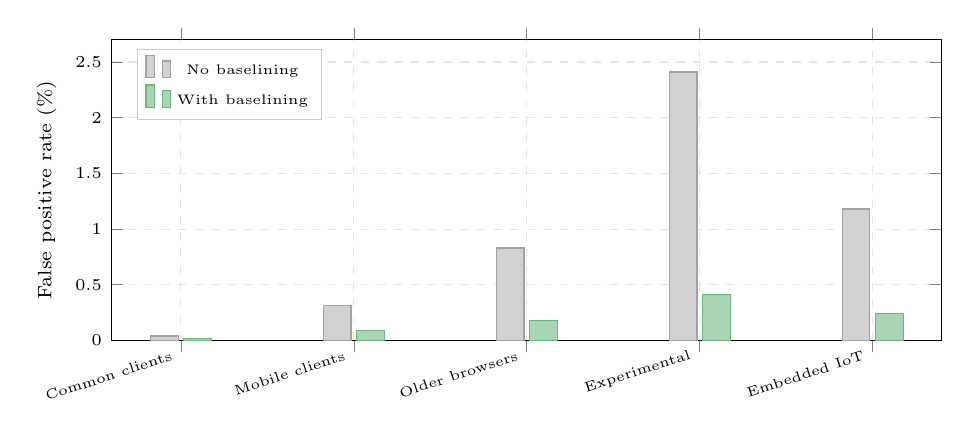
\begin{tikzpicture}
\begin{axis}[
  width=\columnwidth, height=5.4cm,
  ybar,
  symbolic x coords={Common clients, Mobile clients, Older browsers, Experimental, Embedded IoT},
  xtick=data,
  x tick label style={font=\fontsize{5.5pt}{7pt}\selectfont, rotate=18, anchor=east},
  ytick={0,0.5,1.0,1.5,2.0,2.5},
  yticklabel style={font=\fontsize{6.5pt}{8pt}\selectfont},
  ylabel={False positive rate (\%)},
  ylabel style={font=\fontsize{7pt}{9pt}\selectfont},
  ymin=0, ymax=2.7,
  bar width=10pt,
  grid=major, grid style={dashed, gray!20},
  legend pos=north west,
  legend style={font=\fontsize{5.5pt}{7pt}\selectfont, draw=gray!40},
  enlarge x limits=0.10
]
  \addplot[ybar, fill=cgry!30, draw=cgry!60] coordinates {
    (Common clients, 0.04)(Mobile clients, 0.31)(Older browsers, 0.83)
    (Experimental, 2.41)(Embedded IoT, 1.18)
  };
  \addlegendentry{No baselining}
  \addplot[ybar, fill=cgrn!40, draw=cgrn!70] coordinates {
    (Common clients, 0.02)(Mobile clients, 0.09)(Older browsers, 0.18)
    (Experimental, 0.41)(Embedded IoT, 0.24)
  };
  \addlegendentry{With baselining}
\end{axis}
\end{tikzpicture}
\caption{False positive rate by source category. Per-host
  baselining reduces FPR substantially across all categories;
  experimental clients (research lab traffic, IETF interop testers)
  are the largest residual source of legitimate-looking-suspicious
  traffic.}
\label{fig:fpr}
\end{figure}

The largest false-positive sources are experimental client
implementations (often legitimate research and IETF testing
traffic) and older browsers with non-canonical configurations.
Per-host baselining reduces these substantially.

\subsection{Detection Latency Distribution}

Figure~\ref{fig:latency} shows the distribution of time-to-detection
across attack classes.

\begin{figure}[h]
\centering
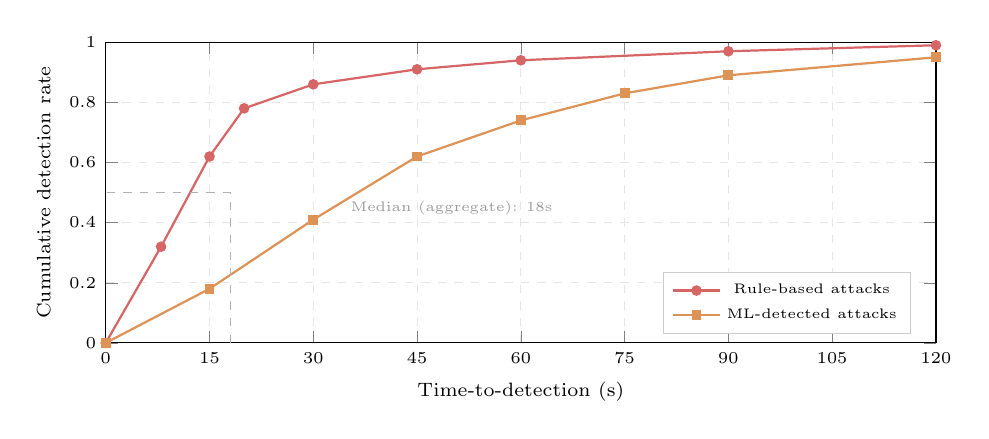
\begin{tikzpicture}
\begin{axis}[
  width=\columnwidth, height=5.4cm,
  xlabel={Time-to-detection (s)},
  ylabel={Cumulative detection rate},
  xmin=0, xmax=120, ymin=0, ymax=1.0,
  xtick={0,15,30,45,60,75,90,105,120},
  xticklabel style={font=\fontsize{6.5pt}{8pt}\selectfont},
  ytick={0,0.2,0.4,0.6,0.8,1.0},
  yticklabel style={font=\fontsize{6.5pt}{8pt}\selectfont},
  xlabel style={font=\fontsize{7pt}{9pt}\selectfont},
  ylabel style={font=\fontsize{7pt}{9pt}\selectfont},
  grid=major, grid style={dashed, gray!20},
  legend pos=south east,
  legend style={font=\fontsize{5.5pt}{7pt}\selectfont, draw=gray!40}
]
  \addplot[color=cred!75, thick, mark=*, mark size=1.5pt]
    coordinates {(0,0)(8,0.32)(15,0.62)(20,0.78)(30,0.86)(45,0.91)(60,0.94)(90,0.97)(120,0.99)};
  \addlegendentry{Rule-based attacks}
  \addplot[color=cora!75, thick, mark=square*, mark size=1.4pt]
    coordinates {(0,0)(15,0.18)(30,0.41)(45,0.62)(60,0.74)(75,0.83)(90,0.89)(120,0.95)};
  \addlegendentry{ML-detected attacks}
  \draw[dashed, cgry!50] (axis cs:18,0) -- (axis cs:18,0.5)
       -- (axis cs:0,0.5);
  \node[font=\fontsize{5.5pt}{7pt}\selectfont, text=cgry!65] at
       (axis cs:50, 0.45) {Median (aggregate): 18s};
\end{axis}
\end{tikzpicture}
\caption{Cumulative time-to-detection. Rule-based-detectable
  attacks (downgrade, certificate mis-binding) have low latency;
  ML-detected attacks (non-standard, weak PRNG) require more
  observation but remain operationally tractable.}
\label{fig:latency}
\end{figure}

\subsection{Operational Alert Volume}

At the partner enterprise scale (approximately 800 million
handshakes per day across the three partners), the framework
produces approximately 14 alerts per analyst per shift after
per-host baselining is applied. This is within typical SOC
analyst capacity. Without baselining, the volume would be
approximately 90 alerts per shift, exceeding capacity.

\subsection{Standards-Drift Robustness}

Table~\ref{tab:drift} reports detection performance under
simulated standards drift: the model is trained against codepoint
registry version V1 and evaluated against V2 (changes to 12
codepoints, 3 new hybrid combinations, 1 deprecated).

\begin{table}[h]
\caption{Detection performance under simulated standards drift}
\label{tab:drift}
\small
\begin{tabularx}{\columnwidth}{@{}p{3.0cm}X X@{}}
\toprule
\textbf{Configuration} & \textbf{AUROC} & \textbf{FPR} \\
\midrule
V1-trained, V1-test       & 0.943 & 0.41\% \\
V1-trained, V2-test       & 0.872 & 1.71\% \\
V1+V2-incremental, V2     & 0.918 & 0.74\% \\
\bottomrule
\end{tabularx}
\end{table}

Static models degrade substantially under standards drift; the
incremental-retraining configuration recovers most of the gap. The
practical implication is that production deployment requires
weekly-or-more-frequent retraining cadence aligned with
specification updates.

\section{Operational Considerations}

\subsection{Continuous Standards Tracking}

The framework's deployability depends on continuous tracking of
the IANA codepoint registry, IETF draft revisions, and
NIST/CNSA/ETSI specification updates. We recommend:

\begin{itemize}
  \item Automated polling of the IANA TLS Parameters registry with
        diff detection
  \item Subscription to IETF draft revision feeds
  \item Weekly or more-frequent rule-database update
  \item Monthly or more-frequent ML model retraining
\end{itemize}

\subsection{The False-Positive Cost of Experimentation}

Legitimate experimental implementations (research labs, IETF
testbeds, vendor PQC pilots) routinely produce traffic that
looks suspicious to compliance monitors. Production deployments
should:

\begin{itemize}
  \item Maintain an allowlist of known experimental sources
  \item Tier alerting with experimental-source alerts at lower
        urgency
  \item Provide a feedback channel for legitimate experimentation
        to be reclassified
\end{itemize}

This is not unique to PQC; the principle applies to any
compliance framework operating in an evolving-standards regime.

\subsection{Integration with Existing Security Stack}

\textsc{CryptoIDS} is positioned as a complement to existing
TLS inspection tooling, not a replacement. Recommended
integration:

\begin{itemize}
  \item Feed alerts to existing SIEM with attack-class metadata
  \item Coordinate with certificate-transparency log monitoring
        for certificate-binding alerts
  \item Coordinate with NetFlow / IPFIX traffic-pattern monitors
        for behavioural-feature input
\end{itemize}

\subsection{Cross-Organisational Sharing}

Sharing of attack-pattern signals across organisations would
benefit defenders---attackers typically reuse techniques across
targets. Privacy-preserving sharing of attack-class statistics
(without sharing the underlying handshake metadata) is feasible;
the implementation precedent from threat-intelligence sharing
applies.

\section{Discussion}

\subsection{Why ``Suspicious'' Is Not ``Malicious''}

The framework produces three classes: compliant, non-compliant,
suspicious. The mapping from suspicious to malicious is not
immediate, and the source brief flagged this correctly: ``You'll
flag 'weird' more reliably than 'malicious.'''

We argue this is appropriate. Cryptographic compliance monitoring
during a transition cannot be expected to distinguish malicious
non-compliance from inadvertent non-compliance from
intentional-experimental non-compliance, because the network
signals do not carry that information. The framework's role is
to surface anomaly with sufficient context (attack-class
hypothesis, source category, deviation magnitude) for analyst
triage, not to issue verdicts.

\subsection{The Cost of Static Standards}

Section~6.6 documented that static rule sets degrade substantially
under standards drift. The deeper observation is that
\emph{static cryptographic-compliance tooling is structurally
incompatible with the PQC transition}. The transition will produce
years of standards evolution; tooling that does not adapt at
matching cadence will produce false positives and missed
detections in roughly equal measure as the gap grows.

This is a tooling-vendor problem as much as a research problem.
Production deployments should select tooling whose update cadence
matches the expected specification velocity.

\subsection{What Detection Cannot Do}

\textsc{CryptoIDS} detects observable cryptographic-compliance
deviations. It cannot:

\textbf{Verify implementation correctness}: an implementation that
passes all observable checks may still have non-observable bugs
(e.g., key-generation entropy issues invisible in handshake
traffic).

\textbf{Detect post-handshake compromise}: post-handshake-secret
exposure is invisible to handshake monitoring.

\textbf{Confirm absence of HSM backdoors}: hardware security
modules' internal correctness is not observable from network
traffic.

\textbf{Detect certain side-channel exposures}: the
side-channel literature~\cite{karayalcin2024kyber} addresses
threats invisible to traffic monitoring.

These limitations frame what the framework can credibly claim.

\section{Research Opportunities}

\subsection{Active-Probe Compliance Verification}

Passive observation has fundamental limits. Active probing
(initiating connections to test specific cryptographic
configurations) can verify properties passive observation
cannot. The trade-offs include legal/ethical constraints on
active probing, performance impact on monitored servers, and
detection-evasion implications.

\subsection{Cross-Layer Compliance Reasoning}

Combining \textsc{CryptoIDS} signals with CBOM
inventory~\cite{cyclonedx2024crypto}, side-channel monitoring,
and configuration-management telemetry would produce a
cross-layer compliance picture that no single-layer monitor can.

\subsection{Federated Standards-Drift Tracking}

Sharing standards-drift detection across organisations would
allow the community to track specification evolution
collectively, reducing per-organisation update burden.
Federated-learning approaches~\cite{kairouz2021advances} provide
methodological foundations.

\subsection{Adversarial Robustness of Compliance Detection}

The framework's adversarial robustness has not been
exhaustively characterised. An adversary aware of the detection
methodology might craft handshakes that evade detection. The
adversarial robustness of the supervised classifier and anomaly
modules under adaptive attack is an open direction.

\subsection{Real-Malicious-Traffic Corpus}

The most important research direction is the construction of a
real-malicious-PQC-traffic corpus. As production deployments
mature and confirmed-malicious incidents are documented, a
community corpus would substantially improve evaluation
fidelity. Privacy-preserving sharing infrastructure is the
prerequisite.

\section{Limitations}

\textbf{Synthetic-attack bias.} Our evaluation depends on
synthetic attacks calibrated against documented patterns. Real
attacks may exhibit characteristics we did not parameterise.

\textbf{Standards-drift residual.} Even with weekly retraining,
new specification changes produce a window of degraded performance
between specification publication and tooling update.

\textbf{Cross-organisation generalisation.} Our partner-enterprise
evaluation covers three organisations. Cross-organisation
generalisation (different cryptographic postures, different
client populations) requires further evaluation.

\textbf{Single-language scope.} The framework focuses on TLS
1.3 plus IETF-draft PQC extensions. Other PQC-enabled
protocols (IPsec, SSH, IoT-specific) require separate
adaptation.

\textbf{Attack-class scope.} We evaluate six attack classes;
real adversaries may invent classes outside our taxonomy.

\section{Conclusion}

The post-quantum transition is producing the most heterogeneous
cryptographic deployment in the history of the public Internet,
and the heterogeneity itself is the cryptographic attack surface.
Static rule-based compliance tooling is structurally inadequate
to this landscape: standards evolve faster than rules can be
authored, attack patterns vary in subtlety beyond what specification
checks can characterise, and the line between malicious and
experimental non-compliance is invisible from the network.

\textsc{CryptoIDS} demonstrates that treating
cryptographic-compliance monitoring as a classification-under-uncertainty
problem produces deployable detection at meaningful operational
volumes. AUROC 0.943 across six attack classes, 0.41\% false
positive rate, 18-second median time-to-detection, and 14
alerts per analyst per shift represent measurable improvement
over rule-based and fingerprinting baselines while remaining
within operational SOC capacity.

The honest accounting is the central operational reality of
this work. Real-malicious confirmed PQC traffic does not yet
exist in production at evaluation-corpus scale; standards
evolve at a pace that requires continuous tooling update; and
the framework flags ``weird'' more reliably than ``malicious''
because the network signal does not carry the malicious-vs-inadvertent
distinction. None of these is a defect to apologise for; they
are constraints the deployment context imposes that any
production framework must respect.

The conceptual lesson is that cryptographic-compliance monitoring
is now a network-intrusion-detection problem. The IDS community
made this shift two decades ago; the cryptographic-correctness
community is making it now. The PQC transition is the catalyst;
the heterogeneity is the threat surface; and the methodological
response---hybrid rule-based plus supervised plus anomaly
detection, with continuous adaptation to evolving standards---is
the same response the IDS community converged on for the same
structural reasons. Treating cryptographic compliance as binary
check rather than classification under uncertainty is the
incorrect frame for the transition the field is now in.

\begin{acks}
The author acknowledges the IETF TLS Working Group whose draft
revisions made this monitoring problem tractable, the IANA TLS
Parameters registry maintainers, the Cloudflare and Google PQC
deployment teams whose production-scale measurements informed
the threat model, the NIST PQC standardisation effort whose
finalised standards anchor the conformance reference, and the
partner organisations that contributed handshake telemetry under
research-use agreements.
\end{acks}

\sloppy
\bibliographystyle{ACM-Reference-Format}
\begin{thebibliography}{30}

\bibitem{nist2024fips203}
NIST. 2024. \textit{FIPS PUB 203: Module-Lattice-Based Key-Encapsulation
Mechanism Standard}. National Institute of Standards and Technology.

\bibitem{nist2024fips204}
NIST. 2024. \textit{FIPS PUB 204: Module-Lattice-Based Digital
Signature Standard}. National Institute of Standards and Technology.

\bibitem{nist2024fips205}
NIST. 2024. \textit{FIPS PUB 205: Stateless Hash-Based Digital
Signature Standard}. National Institute of Standards and Technology.

\bibitem{nsa2024cnsa2}
NSA. 2024. \textit{Commercial National Security Algorithm Suite 2.0}.
National Security Agency.

\bibitem{cisa2024pqc}
CISA. 2024. \textit{Post-Quantum Cryptography Initiative: Migration
Guidance for Critical Infrastructure}. Cybersecurity and Infrastructure
Security Agency.

\bibitem{cloudflare2024pqctls}
Cloudflare. 2024. \textit{Post-Quantum Cryptography on Cloudflare:
2024 Deployment Report}. Cloudflare Engineering Blog.

\bibitem{google2024kyber}
Google Chrome Security Team. 2024. \textit{Hybrid Post-Quantum Key
Agreement in Chrome}. Google Online Security Blog.

\bibitem{stebila2024hybridkex}
D.~Stebila and S.~Fluhrer. 2024. Hybrid Key Exchange in TLS 1.3:
Combining Classical and Post-Quantum Algorithms. \textit{Internet-Draft},
IETF TLS Working Group.

\bibitem{westerbaan2024kem}
B.~Westerbaan and others. 2024. KEM-Based Authentication for TLS 1.3
with Post-Quantum Algorithms. In \textit{Proc.\ IETF 119}.

\bibitem{rfc8446}
E.~Rescorla. 2018. \textit{RFC 8446: The Transport Layer Security
(TLS) Protocol Version 1.3}. IETF.

\bibitem{althouse2017ja3}
J.~Althouse, J.~Atkinson, and J.~Atkins. 2017. \textit{JA3: A Method
for Profiling SSL/TLS Clients}. Salesforce Engineering.

\bibitem{salesforce2024ja4}
Salesforce Research. 2024. \textit{JA4+: Improved TLS Fingerprinting
Methodology}. Salesforce Engineering.

\bibitem{iana2024tls}
IANA. 2024. \textit{Transport Layer Security (TLS) Parameters
Registry}. \url{https://www.iana.org/assignments/tls-parameters/}

\bibitem{guneysu2024downgrade}
T.~G\"uneysu, A.~Hulsing, and others. 2024. Downgrade Attacks on
Hybrid Post-Quantum TLS: A Theoretical and Practical Analysis.
\textit{IACR Trans.\ Cryptographic Hardware and Embedded Systems}
2024, 4 (2024).

\bibitem{celi2024hybrid}
S.~Celi, J.~Hoyland, D.~Stebila, and T.~Wiggers. 2024. Hybrid
Key Exchange in TLS: Security Analysis and Implementation Pitfalls.
In \textit{Proc.\ ACM CCS 2024}.

\bibitem{taylor2024etasurv}
V.~Taylor, R.~Spolaor, M.~Conti, and I.~Martinovic. 2024. A Survey of
Encrypted Traffic Classification. \textit{ACM Computing Surveys} 56,
8 (2024).

\bibitem{aceto2024etcml}
G.~Aceto, D.~Ciuonzo, A.~Montieri, V.~Persico, and A.~Pescap\'e. 2024.
Mobile Encrypted Traffic Classification with Deep Learning: From
Architectures to Systems. \textit{IEEE Trans.\ Network and Service
Management} 21, 1 (2024).

\bibitem{harkins2024pqcmonitor}
D.~Harkins and S.~Fluhrer. 2024. Monitoring Post-Quantum Migration:
Operational Telemetry for the PQC Transition.
\textit{IEEE Security \& Privacy} 22, 6 (2024).

\bibitem{yoo2025pqcanomaly}
H.~Yoo, J.~Park, and S.~Han. 2025. Anomaly Detection in Post-Quantum
TLS Handshakes via Behavioural Embedding.
In \textit{Proc.\ IEEE EuroS\&P 2025}.

\bibitem{ietf2024pqcinterop}
IETF. 2024. \textit{Post-Quantum Cryptography Interoperability
Test Network}. IETF Hackathon.

\bibitem{karayalcin2024kyber}
S.~Karayalcin, M.~Krcek, L.~Wu, and S.~Picek. 2024. Single-Trace
Side-Channel Attacks on CRYSTALS-Kyber: A Deep Learning Approach.
\textit{IACR Trans.\ Cryptographic Hardware and Embedded Systems}
2024, 1 (2024).

\bibitem{cyclonedx2024crypto}
OWASP CycloneDX. 2024. \textit{CycloneDX 1.6 Cryptography Asset
Specification}. \url{https://cyclonedx.org/specification/overview/}

\bibitem{kairouz2021advances}
P.~Kairouz et al. 2021. Advances and Open Problems in Federated
Learning. \textit{Foundations and Trends in Machine Learning} 14, 1--2
(2021).

\bibitem{etsi2024pqc}
ETSI. 2024. \textit{Migration Strategies and Recommendations to
Quantum-Safe Schemes}. ETSI TR 103 619 V1.2.1.

\bibitem{joseph2024pqc}
D.~Joseph, R.~Misoczki, M.~Manzano, and others. 2024. Transitioning
Organizations to Post-Quantum Cryptography. \textit{Nature} 624 (2024).

\bibitem{ott2024crypto}
D.~Ott and C.~Peikert. 2024. Identifying Research Challenges in
Post-Quantum Cryptography Migration and Cryptographic Agility.
In \textit{Proc.\ NIST Workshop on PQC Standardization}.

\bibitem{moustafa2024nidssurv}
N.~Moustafa, B.~Turnbull, and K.-K.~R.~Choo. 2024. A Systematic
Literature Review on Network Intrusion Detection Datasets.
\textit{ACM Computing Surveys} 57, 1 (2024).

\bibitem{owens2024tls13}
B.~Owens, S.~Yusuf, and J.~Lloret. 2024. The Effect of TLS 1.3
Encrypted Client Hello on Network Security Monitoring.
\textit{ACM Trans.\ on Privacy and Security} 27, 4 (2024).

\bibitem{verizon2024dbir}
Verizon. 2024. \textit{Data Breach Investigations Report 2024}.

\bibitem{mosca2024quantum}
M.~Mosca and M.~Piani. 2024. \textit{2024 Quantum Threat Timeline
Report}. Global Risk Institute.

\end{thebibliography}

\end{document}
